\documentclass{article}
\usepackage[utf8]{inputenc}
\usepackage[greek,english]{babel}
\usepackage{alphabeta}
\usepackage{fancyhdr}
\usepackage{listings}
\usepackage{mathtools}
\usepackage{xcolor}
\usepackage{biblatex}
\usepackage[left=2cm,right=2cm]{geometry}

\lstset {
        basicstyle=\ttfamily,
        columns=fullflexible,
        breaklines=true,
        keepspaces=true
}

\title{Σχεδίαση Ψηφιακών Συστημάτων - Εργασία Θεωρίας (Μέρος 6)}
\author{Χρήστος Μαργιώλης}
\date{Ιούλιος 2020}

\begin{document}

\begin{titlepage}
        \maketitle
\end{titlepage}

\renewcommand{\contentsname}{Περιεχόμενα}
\tableofcontents

\section{Κώδικας και τεκμηρίωση}

\subsection{\lstinline{reg.vhd}}

Το παρακάτω κύκλωμα υλοποιεί έναν καταχωρητή. Ο κώδικας είναι παραμετροποιημένος
για να μπορεί να μετατραπεί στο επόμενο μέρος σε 32-bit χωρίς αλλαγές. \\

\lstinputlisting[language=VHDL]{../reg.vhd}
\pagebreak

\subsection{\lstinline{reg_tb.vhd}}

Testbench για τον καταχωρητή. \\

\lstinputlisting[language=VHDL]{../reg_tb.vhd}
\pagebreak

\subsection{\lstinline{regfile.vhd}}

Το παρακάτω κύκλωμα υλοποιεί ένα register file. \\

\lstinputlisting[language=VHDL]{../regfile.vhd}
\pagebreak

\subsection{\lstinline{regfile_tb.vhd}}

Testbench για το register file. \\

\lstinputlisting[language=VHDL]{../regfile_tb.vhd}
\pagebreak

\subsection{\lstinline{regfile_ext.vhd}}

Το παρακάτω κύκλωμα υλοποιεί ένα register file με δύο επιπλέον θύρες. \\

\lstinputlisting[language=VHDL]{../regfile_ext.vhd}
\pagebreak

\subsection{\lstinline{regfile_ext_tb.vhd}}

Testbench για το register file με δύο επιπλέον θύρες. \\

\lstinputlisting[language=VHDL]{../regfile_ext_tb.vhd}
\pagebreak

\section{Εκτέλεση}

\subsection{\lstinline{reg_tb}}
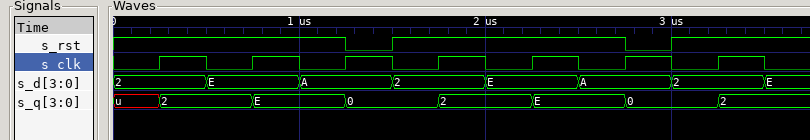
\includegraphics[width=\textwidth]{res/reg.png}

\subsection{\lstinline{regfile_tb}}
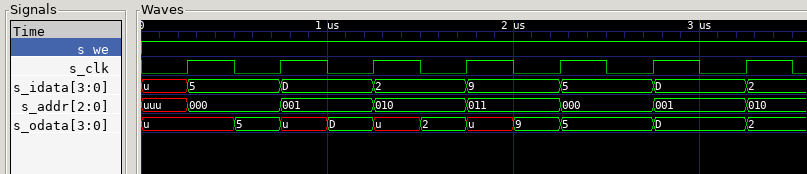
\includegraphics[width=\textwidth]{res/regfile.png}

\subsection{\lstinline{regfile_ext_tb}}
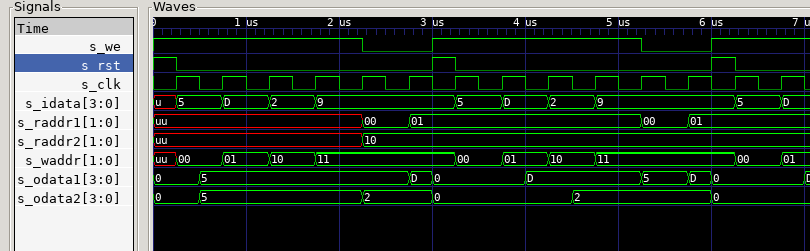
\includegraphics[width=\textwidth]{res/regfile_ext.png}

\end{document}
